%% Figure 3 (pgfplots): Layerwise feature learning across the full two-block Transformer (clean spacing & outward ticks).
\definecolor{stepc}{HTML}{0072B2}\definecolor{outc}{HTML}{D55E00}\definecolor{theoc}{HTML}{1E7E4E}
\definecolor{modelc}{HTML}{6A3D9A}\definecolor{mutedc}{HTML}{6E6E6E}
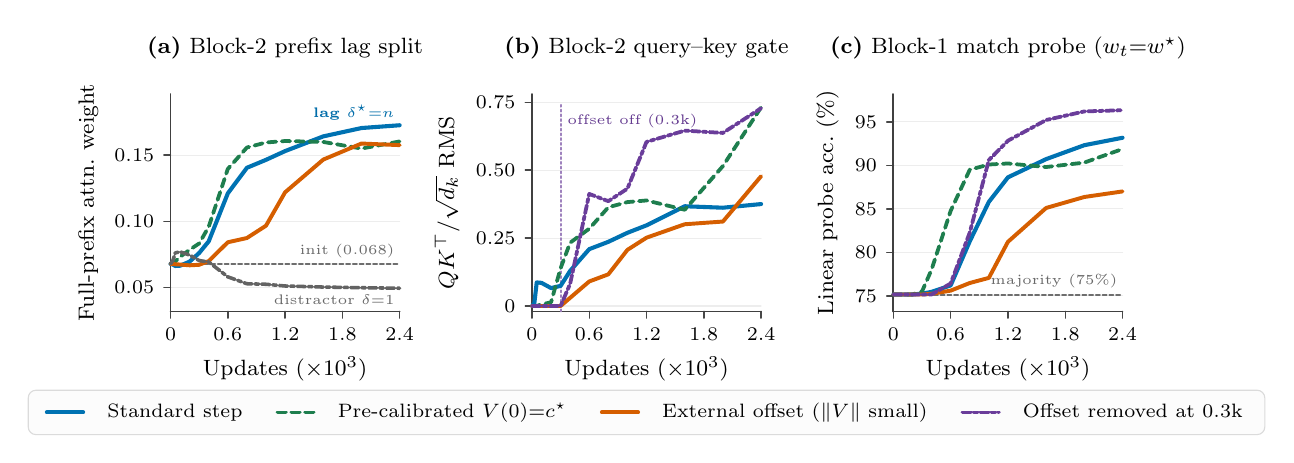
\begin{tikzpicture}[line cap=round, line join=round]
\pgfplotsset{
  every axis/.style={
    scale only axis,
    width=0.240\textwidth,
    height=2.76cm,
    axis line style={black!75, line width=0.64pt},
    tick align=outside,
    tickwidth=2.4pt,
    tick style={black!72, line width=0.52pt},
    tick label style={font=\scriptsize},
    label style={font=\footnotesize},
    ylabel style={yshift=-1pt},
    xlabel style={yshift=1pt},
    title style={font=\footnotesize, at={(0.5,1.04)}, anchor=south},
    axis x line*=bottom,
    axis y line*=left,
    ymajorgrids,
    major grid style={black!7, line width=0.38pt},
    clip=false
  },
  every axis plot/.append style={line width=1.44pt}
}

% (a) Block-2 full-prefix lag separation: target lag \delta^* = n vs nearest distractor \delta = 1
\begin{axis}[
  name=fa,
  title={\textbf{(a)} Block-$2$ prefix lag split},
  xlabel={Updates ($\times 10^3$)},
  ylabel={Full-prefix attn.\ weight},
  xmin=0, xmax=2.4, ymin=0.032, ymax=0.196,
  xtick={0,0.6,1.2,1.8,2.4},
  ytick={0.05,0.10,0.15},
  yticklabels={$0.05$,$0.10$,$0.15$}
]
  \addplot[mutedc, densely dotted, line width=0.75pt, domain=0:2.4, samples=2, forget plot] {0.0679};
  \node[anchor=south east, font=\tiny, text=mutedc!95!black, inner sep=1pt] at (axis cs:2.38,0.070) {init ($0.068$)};

  \addplot[stepc, solid, line width=1.48pt] coordinates {
    (0.000,0.0679) (0.025,0.0674) (0.050,0.0663) (0.100,0.0665) (0.200,0.0696)
    (0.300,0.0761) (0.400,0.0849) (0.600,0.1211) (0.800,0.1404) (1.000,0.1464)
    (1.200,0.1530) (1.600,0.1641) (2.000,0.1704) (2.400,0.1725)
  };
  \node[anchor=south east, font=\tiny\bfseries, text=stepc!95!black, inner sep=1pt] at (axis cs:2.38,0.174) {lag $\delta^\star{=}n$};

  \addplot[theoc, densely dashed, line width=1.36pt] coordinates {
    (0.000,0.0679) (0.025,0.0682) (0.050,0.0698) (0.100,0.0732) (0.200,0.0785)
    (0.300,0.0833) (0.400,0.0959) (0.600,0.1395) (0.800,0.1557) (1.000,0.1595)
    (1.200,0.1606) (1.600,0.1599) (2.000,0.1549) (2.400,0.1603)
  };

  \addplot[outc, solid, line width=1.42pt] coordinates {
    (0.000,0.0679) (0.025,0.0678) (0.050,0.0676) (0.100,0.0674) (0.200,0.0668)
    (0.300,0.0672) (0.400,0.0700) (0.600,0.0842) (0.800,0.0874) (1.000,0.0967)
    (1.200,0.1219) (1.600,0.1466) (2.000,0.1587) (2.400,0.1575)
  };

  \addplot[mutedc!90!black, densely dashdotted, line width=1.28pt] coordinates {
    (0.000,0.0679) (0.025,0.0705) (0.050,0.0762) (0.100,0.0770) (0.200,0.0745)
    (0.300,0.0704) (0.400,0.0693) (0.600,0.0581) (0.800,0.0529) (1.000,0.0525)
    (1.200,0.0512) (1.600,0.0504) (2.000,0.0499) (2.400,0.0495)
  };
  \node[anchor=north east, font=\tiny, text=mutedc!95!black, inner sep=1pt] at (axis cs:2.38,0.047) {distractor $\delta{=}1$};
\end{axis}

% (b) Block-2 query-key score RMS opening across plateau
\begin{axis}[
  name=fb,
  at={(fa.east)}, anchor=west, xshift=1.68cm,
  title={\textbf{(b)} Block-$2$ query--key gate},
  xlabel={Updates ($\times 10^3$)},
  ylabel={$QK^\top/\sqrt{d_k}$ RMS},
  xmin=0, xmax=2.4, ymin=-0.02, ymax=0.78,
  xtick={0,0.6,1.2,1.8,2.4},
  ytick={0,0.25,0.50,0.75},
  yticklabels={$0$,$0.25$,$0.50$,$0.75$},
  legend style={
    at={(0.5,-0.36)},
    anchor=north,
    legend columns=4,
    font=\scriptsize,
    draw=black!14,
    fill=black!1.2,
    rounded corners=2.8pt,
    inner xsep=6pt,
    inner ysep=2.6pt,
    column sep=6pt,
    cells={anchor=west},
    /tikz/every even column/.append style={column sep=10pt}
  },
  legend image code/.code={
    \draw[#1] (0cm,0cm) -- (0.46cm,0cm);
  }
]
  \draw[modelc!65, densely dotted, line width=0.72pt] (axis cs:0.30,-0.02) -- (axis cs:0.30,0.74);
  \node[anchor=west, font=\tiny, text=modelc!92!black, inner sep=1pt] at (axis cs:0.34,0.68) {offset off ($0.3$k)};

  \addplot[stepc, solid, line width=1.48pt] coordinates {
    (0.000,0.0000) (0.025,0.0100) (0.050,0.0868) (0.100,0.0852) (0.200,0.0660)
    (0.300,0.0740) (0.400,0.1292) (0.600,0.2093) (0.800,0.2362) (1.000,0.2695)
    (1.200,0.2969) (1.600,0.3672) (2.000,0.3618) (2.400,0.3752)
  };
  \addlegendentry{Standard step}

  \addplot[theoc, densely dashed, line width=1.36pt] coordinates {
    (0.000,0.0000) (0.025,0.0000) (0.050,0.0003) (0.100,0.0059) (0.200,0.0136)
    (0.300,0.1388) (0.400,0.2331) (0.600,0.2845) (0.800,0.3635) (1.000,0.3825)
    (1.200,0.3885) (1.600,0.3543) (2.000,0.5151) (2.400,0.7314)
  };
  \addlegendentry{Pre-calibrated $V(0){=}c^\star$}

  \addplot[outc, solid, line width=1.42pt] coordinates {
    (0.000,0.0000) (0.025,0.0000) (0.050,0.0000) (0.100,0.0000) (0.200,0.0000)
    (0.300,0.0000) (0.400,0.0302) (0.600,0.0903) (0.800,0.1166) (1.000,0.2066)
    (1.200,0.2515) (1.600,0.3009) (2.000,0.3109) (2.400,0.4777)
  };
  \addlegendentry{External offset ($\|V\|$ small)}

  \addplot[modelc, densely dashdotted, line width=1.36pt] coordinates {
    (0.000,0.0000) (0.025,0.0000) (0.050,0.0000) (0.100,0.0000) (0.200,0.0000)
    (0.300,0.0000) (0.400,0.0818) (0.600,0.4126) (0.800,0.3859) (1.000,0.4320)
    (1.200,0.6041) (1.600,0.6456) (2.000,0.6371) (2.400,0.7280)
  };
  \addlegendentry{Offset removed at $0.3$k}
\end{axis}

% (c) Block-1 match-bit feature probe accuracy (w_t = w^*)
\begin{axis}[
  name=fc,
  at={(fb.east)}, anchor=west, xshift=1.68cm,
  title={\textbf{(c)} Block-$1$ match probe ($w_t{=}w^\star$)},
  xlabel={Updates ($\times 10^3$)},
  ylabel={Linear probe acc.\ (\%)},
  xmin=0, xmax=2.4, ymin=73.2, ymax=98.2,
  xtick={0,0.6,1.2,1.8,2.4},
  ytick={75,80,85,90,95},
  yticklabels={$75$,$80$,$85$,$90$,$95$}
]
  \addplot[mutedc, densely dotted, line width=0.75pt, domain=0:2.4, samples=2, forget plot] {75.14};
  \node[anchor=south east, font=\tiny, text=mutedc!95!black, inner sep=1pt] at (axis cs:2.38,75.5) {majority ($75\%$)};

  \addplot[stepc, solid, line width=1.48pt] coordinates {
    (0.000,75.1490) (0.025,75.1490) (0.050,75.1490) (0.100,75.1490) (0.200,75.1490)
    (0.300,75.2450) (0.400,75.4500) (0.600,76.1940) (0.800,81.2660) (1.000,85.7980)
    (1.200,88.6250) (1.600,90.7220) (2.000,92.3230) (2.400,93.1790)
  };

  \addplot[theoc, densely dashed, line width=1.36pt] coordinates {
    (0.000,75.1445) (0.025,75.1445) (0.050,75.1445) (0.100,75.1445) (0.200,75.1564)
    (0.300,75.4955) (0.400,78.0118) (0.600,84.7673) (0.800,89.4991) (1.000,90.1000)
    (1.200,90.2218) (1.600,89.8118) (2.000,90.3227) (2.400,91.8855)
  };

  \addplot[outc, solid, line width=1.42pt] coordinates {
    (0.000,75.1445) (0.025,75.1445) (0.050,75.1445) (0.100,75.1445) (0.200,75.1445)
    (0.300,75.1445) (0.400,75.2318) (0.600,75.5918) (0.800,76.4709) (1.000,77.0573)
    (1.200,81.2091) (1.600,85.1027) (2.000,86.3655) (2.400,87.0045)
  };

  \addplot[modelc, densely dashdotted, line width=1.36pt] coordinates {
    (0.000,75.1490) (0.025,75.1490) (0.050,75.1490) (0.100,75.1490) (0.200,75.1490)
    (0.300,75.1490) (0.400,75.1490) (0.600,76.4140) (0.800,82.2740) (1.000,90.6120)
    (1.200,92.8390) (1.600,95.2220) (2.000,96.2090) (2.400,96.3470)
  };
\end{axis}
\end{tikzpicture}
